In this chapter, we show that the YB-isoTPS ansatz introduced in Chapter \ref{chap:isoTPS_alternative_canonical_form} is able to exactly represent the ground state of the Toric Code Model, as was also shown for MM-isoTPS \cite{cite:isometric_tensor_network_representation_of_string_net_liquids}. We first give a brief introduction to the Toric Code model in Section \ref{sec:the_toric_code_model} and show how the ground state can be derived analytically. We then discuss how this ground state can be represented as a YB-isoTPS in Section \ref{sec:representing_the_toric_code_gs_with_YB_isoTPS}, following \cite{cite:isometric_tensor_network_representation_of_string_net_liquids}.

\section{The Toric Code Model}
\label{sec:the_toric_code_model}
The Toric Code is an exactly soluble spin model with $\mathbb{Z}_2$ topological order that was introduced by Alexei Kitaev \cite{cite:fault_tolerant_quantum_computation_by_anyons}. The model is defined on the square lattice with periodic boundary conditions, where on each edge of the lattice there sits a spin-1/2 degree of freedom. Two operators are introduced, the \textit{star operators}
\begin{equation}
	\label{eq:star_operator}
	\hat{A}_+ \coloneqq \sum_{j\in+}\hat{\sigma}_j^z
\end{equation}
and the \textit{plaquette operators}
\begin{equation}
	\label{eq:plaquette_operator}
	\hat{B}_{\scalebox{0.6}{$\square$}} \coloneqq \sum_{j\in \scalebox{0.6}{$\square$}} \hat{\sigma}_j^x,
\end{equation}
where the sums are performed over the four spins connected in a star or plaquette pattern respectively (see Figure \figref{fig:toric_code_star_and_plaquette_operators}) and $\hat{\sigma}_j^x, \hat{\sigma}_j^z$ are Pauli matrices. The Hamiltonian of the Toric Code model is then defined as
\begin{equation}
	\label{eq:toric_code_hamiltonian}
	H_\text{TC} \coloneqq -\sum_+\hat{A}_+ - \sum_{\scalebox{0.6}{$\square$}}\hat{B}_{\scalebox{0.6}{$\square$}},
\end{equation}
where the sums go over all possible stars and plaquettes respectively. Because an arbitrary star and plaquette operator share either two or zero spins, all terms of the Hamiltonian commute and it is thus possible to find the ground state of the model by diagonalizing all terms simultaneously. To diagonalize the star operators $\hat{A}_+$ we choose a basis of $\hat{\sigma}_z$-eigenstates $\ket{i} \in \left\{\ket{\uparrow}, \ket{\downarrow}\right\}$ with eigenvalues $\left\langle\hat{\sigma}_z\right\rangle_i = s_i = \pm 1$ for each spin $i$. In this basis every star operator is diagonal with eigenvalues
\begin{equation}
	\label{eq:toric_code_star_operator_expectation value}
	\langle \hat{A}_+\rangle = \prod_{j\in+}s_j \in \left\{1, -1\right\}.
\end{equation}
To obtain the expectation value $\langle \hat{A}_+\rangle = 1$, the number of spins in the down state $s_j = -1$ around the vertex $+$ must be even. Basis states $\ket{s}$ that give an expectation value of $1$ for every star operator simultaneously are thus the states with an even number of down-spins around every vertex,
\begin{equation}
	\label{eq:toric_code_A_operator_condition}
	\ket{s} = \ket{s_1} \otimes \dots \otimes \ket{s_N}, \quad \prod_{j\in+}s_j = 1 \,\,\,\,\forall +.
\end{equation}
The plaquette operator $\hat{B}_{\scalebox{0.6}{$\square$}}$ acts on a basis state by flipping all spins around the plaquette $\scalebox{0.6}{$\square$}$. Because a plaquette and a star share either zero or two spins, applying an plaquette operator to a state $\ket{s}$ satisfying condition \eqref{eq:toric_code_A_operator_condition} produces a state $\ket{s^\prime}$ that again satisfies \eqref{eq:toric_code_A_operator_condition}, and applying the plaquette operator a second time produces the initial state $\ket{s}$. If we now take the equal weighted superposition $\ket{\Psi} = \left(\ket{s}+\ket{s^\prime}\right)/\sqrt{2}$, the expectation value of $\hat{B}_{\scalebox{0.6}{$\square$}}$ becomes $\langle \hat{B}_{\scalebox{0.6}{$\square$}}\rangle = 1$.
The ground state of the Hamiltonian \eqref{eq:toric_code_hamiltonian} is thus given by the equal weighted superposition of all basis states satisfying condition \eqref{eq:toric_code_A_operator_condition}. \par
One can show that the ground state can be written as
\begin{equation}
	\ket{\Psi_0} \propto \prod_{\scalebox{0.6}{$\square$}}\left(\id + \hat{B}_{\scalebox{0.6}{$\square$}}\right) \ket{\uparrow} \otimes \dots \otimes \ket{\uparrow}.
\end{equation}
Note that this is also the ground state for the model if open boundary conditions are chosen instead. \par
For periodic boundary conditions, which is equivalent to putting the model on a torus, one can further show that the ground state is fourfold topologically degenerate. To move from one degenerate section of the Hilbert space to another one must apply a string of operators, wrapping once around the torus. This is a highly non-local operation. Because perturbations are usually local, the toric code model can be interpreted as a form of hardware level error correction. The toric code is considered a topological quantum error correction code and can in theory be used for quantum memory. One can further implement quantum gates acting on the 4-dimensional ground state space by locally creating a pair of anyonic excitations, moving one of the excitations around the torus, and annihilating it with the other one \cite{cite:fault_tolerant_quantum_computation_by_anyons}. Unfortunately, the gates that can be implemented as such do not form a complete state set and thus do not allow for universal quantum computing. Nevertheless, the Toric code is an important model for the study of topological order and anyonic excitations.
\begin{figure}
	\centering
	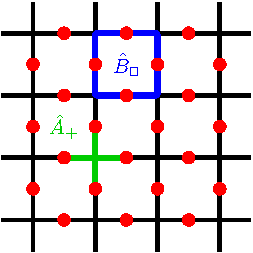
\includegraphics[scale=1]{figures/tikz/toric_code/toric_code_general/toric_code_general.pdf}
	\caption{The Toric Code model is defined on the square lattice with spin-1/2 degrees of freedom living on the edges. the star and plaquette operators \eqref{eq:star_operator} and \eqref{eq:plaquette_operator} act on the four spins arranged in a star or plaquette shape respectively.}
	\label{fig:toric_code_star_and_plaquette_operators}
\end{figure}


\section{Representing the Toric Code Ground State with YB-isoTPS}
\label{sec:representing_the_toric_code_gs_with_YB_isoTPS}
\begin{figure}
	\centering
	\subcaptionbox{\label{fig:toric_code_doubling_dof}}
	{%
		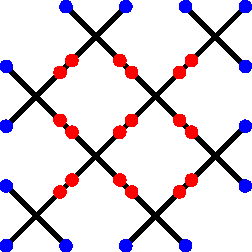
\includegraphics[scale=1]{figures/tikz/toric_code/peps_representation/peps_representation_a.pdf}
	}
	\quad
	\subcaptionbox{\label{fig:toric_code_PEPS_representation_tensor_definitions}}
	{%
		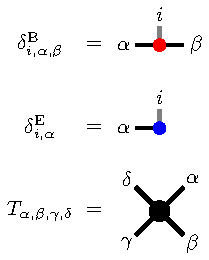
\includegraphics[scale=1]{figures/tikz/toric_code/peps_representation/peps_representation_b.pdf}
	}
	\quad
	\subcaptionbox{\label{fig:toric_code_PEPS_representation}}
	{%
		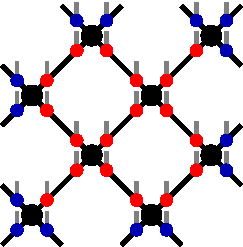
\includegraphics[scale=1]{figures/tikz/toric_code/peps_representation/peps_representation_c.pdf}
	}
	\caption{(a) To represent the Toric Code ground state as a PEPS we start by doubling the local degrees of freedom on each edge in the bulk. Bulk spins are denoted in red, while boundary spins are coloured blue. (b) Tensor diagrams of the tensors $\delta^\text{B}$, $\delta^\text{E}$ and $T$ introduced in the text. (b) The PEPS representation of the Toric Code ground state before contracting the tensors at each vertex, made up from the tensors (b).}
	\label{fig:toric_code_doubling_dof_and_PEPS_representation}
\end{figure}
\begin{figure}
	\centering
	\savebox{\largestimage}{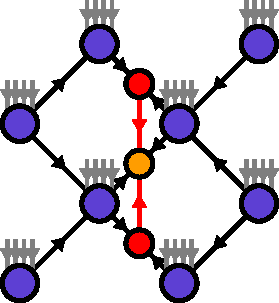
\includegraphics[scale=1]{figures/tikz/toric_code/YB_isoTPS_representation/YB_isoTPS_representation_a.pdf}}
	\subcaptionbox{\label{fig:toric_code_YB_isoTPS_representation}}
	{%
		\usebox{\largestimage}
	}
	\quad\quad\quad
	\subcaptionbox{\label{fig:toric_code_YB_isoTPS_representation_tensor_definitions}}
	{%
		\raisebox{\dimexpr.5\ht\largestimage-.5\height}
		{%
			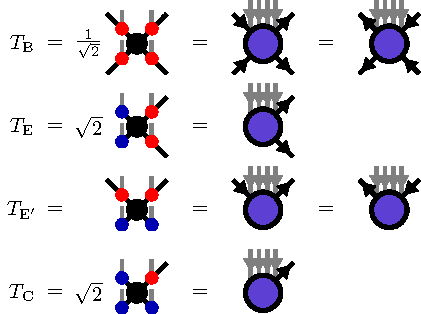
\includegraphics[scale=1]{figures/tikz/toric_code/YB_isoTPS_representation/YB_isoTPS_representation_b.pdf}
		}
	}
	\caption{The PEPS in figure \protect\figref{fig:toric_code_PEPS_representation} can be transformed to the disoTPS (a) by normalizing the tensors as shown in (b). Note that the tensors $T_\text{E}^\prime$ at the top and bottom edges of the lattice need a different normalization than the tensors $T_\text{E}$ at the left and right edges.}
	\label{fig:toric_code_YB_isoTPS}
\end{figure}
We will now derive the disoTPS corresponding to the Toric Code ground state on a square lattice with open boundary condition. We choose rough boundary conditions \cite{cite:models_for_gapped_boundaries_and_domain_walls}, fixing all boundary spins to the state $\left(\ket{\uparrow} + \ket{\downarrow}\right)/\sqrt{2}$. As shown in \cite{cite:isometric_tensor_network_representation_of_string_net_liquids}, the Toric Code ground state can be represented exactly as a PEPS with bond dimension $D = 2$. One can construct such a PEPS easily by first doubling the Hilbert space on each edge as $\ket{s_i} \rightarrow \ket{s_i}\otimes\ket{s_i}$, which we show in Figure \figref{fig:toric_code_doubling_dof}. In the PEPS representation the physical degrees of freedom on each edge in the bulk are then carried by two identical tensors $\delta^\text{B}\in\mathbb{R}^{2\times2\times2}$,
\begin{equation}
	\delta^\text{B}{i,\alpha,\beta} = \begin{cases}
		1 &\text{if }i=\alpha=\beta\\
		0 &\text{else}
	\end{cases},
\end{equation}
as shown in Figure \figref{fig:toric_code_PEPS_representation_tensor_definitions}. The boundary spins are represented by tensors $\delta_E\in\mathbb{R}^{2\times2}$,
\begin{equation}
	\delta^\text{E}{i,\alpha} = \begin{cases}
		1 &\text{if }i=\alpha\\
		0 &\text{else}
	\end{cases}.
\end{equation}
We proceed by associating each vertex with the spins on the four connected edges and connect the corresponding tensors $\delta^\text{B}$ and $\delta^\text{E}$ with a tensor $T\in\mathbb{R}^{2\times2\times2\times2}$ that is placed on each vertex,
\begin{equation}
	T_{i,j,k,l} = \begin{cases}
		1 & \text{if } \left(i+j+k+l\right)\mod2 = 0 \\
		0 & \text{else}
	\end{cases}.
\end{equation}
This tensor ensures that all states with an odd number of down spins around a vertex have an amplitude of zero, satisfying condition \eqref{eq:toric_code_A_operator_condition}. \par
We arrive at the PEPS in Figure \figref{fig:toric_code_PEPS_representation}. Each basis state satisfying condition \eqref{eq:toric_code_A_operator_condition} results in the same amplitude when contracting the PEPS, while basis states violating the condition vanish. Thus, the PEPS represents the ground state of the Toric Code. \par
We now want to transform the PEPS into a disoTPS. This can be easily done by choosing the correct normalization for the vertex tensors, which transforms them into isometries as shown in Figure \figref{fig:toric_code_YB_isoTPS_representation_tensor_definitions}. Note that different normalizations need to be chosen for tensors at the corners, edges, and in the bulk. For each vertex tensor we can choose the isometry direction to point to the left or to the right respectively, allowing us to place the orthogonality hypersurface anywhere in the lattice. As a last step, the tensors of the orthogonality hypersurface must be specified. The two spins that are connected to a tensor $W$ of the orthogonality hypersurface must be in the same local state, since they were created by doubling the local degree of freedom. This constraint can be enforced by setting $W\in\mathbb{R}^{2\times1\times2\times1}$ to
\begin{equation}
	W_{\alpha,\nu,\beta,\mu} = \frac{\delta_{\alpha,\beta}}{\sqrt{2}}
\end{equation} 
with dummy indices $\nu, \mu$ of bond dimension $1$. Trivially, the tensors $W$ fulfil the isometry condition. We can again choose the direction of isometry to point either up or down for every $W$-tensor, allowing us to place the orthogonality center freely along the orthogonality hypersurface.\par
We have thus found an exact disoTPS representation of the Toric Code ground state with $D = 2$ and $\chi= 1$, similar to the construction done in \cite{cite:isometric_tensor_network_representation_of_string_net_liquids} for isoTPS. The final network is depicted in Figure \figref{fig:toric_code_YB_isoTPS_representation}. We test the different algorithms for the YB move on the Toric Code ground state on a $5\times5$ lattice. All algorithms are able to move the orthogonality surface exactly up to computational accuracy. This however only works well if a good initialization is chosen for the disentangling unitary. We choose an initialization based on an SVD, see \cite{cite:isometric_tensor_network_states_in_two_dimensions, cite:efficient_simulation_of_dynamics_in_two_dimensional_quantum_spin_systems} or our implementation \cite{cite:github_YB_isoTPS}.